%% Latex Template for 16-720J student reports
%% You should maintain the template format wherever practical
%% Gary Overett 2015

\documentclass[12pt]{article}
\usepackage{amsmath}
\usepackage{amssymb}
\usepackage{amsthm}
\usepackage{amscd}
\usepackage{amsfonts}
\usepackage{graphicx}
\usepackage{subcaption}
\usepackage{fancyhdr}
\usepackage{tablefootnote}
\usepackage{subcaption}
\usepackage[table]{xcolor}
\usepackage{array,multirow}
\usepackage{hyperref}
\usepackage{enumerate}
\usepackage{bm}

\topmargin-2cm
\textheight+23cm

\textwidth6.5in

\setlength{\topmargin}{0in} \addtolength{\topmargin}{-\headheight}
\addtolength{\topmargin}{-\headsep}

\setlength{\oddsidemargin}{0in}

\oddsidemargin  0.0in \evensidemargin 0.0in 

\newcounter{list}

\begin{document}

\title{16720J: Homework 1 - Planar Homographies}

\author{Name - Wenbo Zhao}

\date{September 24, 2015}

\maketitle

\setcounter{section}{2}

\section{Planar Homographies: Theory (40pts)}

\subsection{(10pts)}

Prove that there exists an $\bm{ H}$ that the satisfies homography equation.
\\
The easiest way to show this is to assume \emph{the points are on the same $Z=0$ plane}. Then the points in the plane are of the form $\bm{[X\,Y\,1]^T}$

Therefore, the original equations for $\bm{p1}$ and $\bm{p2}$:

\begin{equation}
  p_1 \equiv \left[ \begin{matrix}
      m_{11} & m_{12} & m_{13} & m_{14} \\
      m_{21} & m_{22} & m_{23} & m_{24} \\
      m_{31} & m_{32} & m_{33} & m_{34}
    \end{matrix} \right]_1
\left[ \begin{matrix}
X\\
Y\\
Z\\
1
\end{matrix} \right]
\end{equation}

\begin{equation}
  p_2 \equiv \left[ \begin{matrix}
      m_{11} & m_{12} & m_{13} & m_{14} \\
      m_{21} & m_{22} & m_{23} & m_{24} \\
      m_{31} & m_{32} & m_{33} & m_{34}
    \end{matrix} \right]_2
\left[ \begin{matrix}
X\\
Y\\
Z\\
1
\end{matrix} \right]
\end{equation}

can be written as:
\begin{equation}
 p_1 \equiv \left[ \begin{matrix}
      m_{11} & m_{12} & m_{14} \\
      m_{21} & m_{22} & m_{24} \\
      m_{31} & m_{32} & m_{34}
    \end{matrix} \right]_1
\left[ \begin{matrix}
X\\
Y\\
1
\end{matrix} \right]
\end{equation}

\begin{equation}
 p_2 \equiv \left[ \begin{matrix}
      m_{11} & m_{12} & m_{14} \\
      m_{21} & m_{22} & m_{24} \\
      m_{31} & m_{32} & m_{34}
    \end{matrix} \right]_2
\left[ \begin{matrix}
X\\
Y\\
1
\end{matrix} \right]
\end{equation}

therefore there exists an $\bm{H}$ where

\begin{equation}
  p_2 \equiv M_2 P \equiv M_2 M^{-1}_1 p_1, \ H = M_2 M^{-1}_1.
\end{equation}

When does this fail?

A: When one of the projection matrices $M_2$ or $M_1$ equals to $0$, \emph{i.e.} $det(M_1) = 0$ or $det(M_2) =0$.


\pagebreak

\subsection{(10pts)}
\label{rot}

Prove that there exists an $\bm{H}$ that satisfies homography equation given two cameras separated by a pure rotation.

\begin{equation*}
  p_1 = K_1 [I\,0] P
\end{equation*}
\begin{equation}
  p_2 = K_2 [R\, 0] P
\end{equation}

Now you are trying to find that the H exists. It will be a good idea to try to manipulate these expressions in the
direction of some expression

\begin{equation*}
  p_1 = K_1 P
\end{equation*}
\begin{equation}
  p_2 = K_2 R P
\end{equation}

so
\begin{equation*}
  p_2 = K_2 R K_1^{-1} p_1
\end{equation*}

\begin{equation}
  H \equiv K_2 R K_1^{-1}.
\end{equation}



\subsection{(5pts)}

From Section \ref{rot}

\begin{equation}
  H \equiv K_2 R K_1^{-1} \equiv K R K^{-1}\ (\textup{when $K$ is constant})
\end{equation}

therefore

\begin{equation}
  H^2 \equiv K R K^{-1} K R K^{-1} \equiv K R^2 K^{-1},
\end{equation}
which indicating a rotation of $2\theta$.

\subsection{(5pts)}

Why is the planar homography not completely sufficient to map any arbitrary scene image to another viewpoint?

The planar homography maps points that are on the world plane to another viewpoint, not points on an arbitrary plane, except that the different viewpoints are got from camera purely rotating about its center. 



\subsection{(5pts)}

We have a set of points $\bm{p^i_1}$ in an image taken by camera $\bm{C_1}$ and points $\bm{p^i_2}$ in an image taken by
$\bm{C_2}$. Suppose we know there exists an unknown homography $\bm{H}$ such that

\begin{equation}
\bm{p^i_1 \equiv Hp^i_2}
\label{eq:p1Hp2}
\end{equation}

Assume the points are homogeneous coordinates in the form $\bm{p^i_j = (x^i_j,y^i_j,1)^T}$. For a single point pair, write a matrix
equation of the form
\begin{equation}
  \bm{Ah = 0}
\end{equation}

Where $\bm{h}$ is a vector of the elements of $\bm{H}$ and $\bm{A}$ is a matrix composed of the point coordinates.

HINT: we are thinking about the relation

\begin{equation}
\bm{p_1 \equiv Hp_2}
\end{equation}

but we want something in the form $Ax = 0$

Now look at the lecture notes for ``things $=0$''.

Good luck!

\textbf{Solution}:\\
Eq.~\ref{eq:p1Hp2} can be written as
\begin{equation}
 \left[ \begin{matrix}
	 x_1^i\\
	 y_1^i\\
	 1
 \end{matrix} \right]
 \equiv 
 \left[ \begin{matrix}
     h_{11} & h_{12} & h_{13} \\
     h_{21} & h_{22} & h_{23} \\
     h_{31} & h_{32} & h_{33}
 \end{matrix} \right]
 \left[ \begin{matrix}
	 x_2^i\\
	 y_2^i\\
	 1
 \end{matrix} \right]
\end{equation}

After writing down the nonlinear relations and linearizing, we have
\begin{equation}
\left[ \begin{matrix}
    [x_2^i\ y_2^i\ 1] & \mathbf{0} & -x_1^i[x_2^i\ y_2^i\ 1] \\
    \mathbf{0} & [x_2^i\ y_2^i\ 1] & -y_1^i[x_2^i\ y_2^i\ 1]
 \end{matrix} \right]
 \left[ \begin{matrix}
	 h_{11}\\
	 h_{12}\\
	 h_{13}\\
	 h_{21}\\
	 h_{22}\\
	 h_{23}\\
	 h_{31}\\
	 h_{32}\\
	 h_{33}
 \end{matrix} \right] = \mathbf{0}
\end{equation}
1. How many elements are there in $h$?\\
\indent 9.\\
2. How many point pairs are required to solve this system?\\
\indent 4 pairs.\\
3. Show how to estimate the elements in $h$ using the Rayleigh Quotient Theorem mentioned in class to find a solution to minimize this homogeneous linear least squares system.\\
\begin{equation*}
\begin{split}
 \textup{min}\ h^T A^T A h \\
 s.t.\ \|h\|_1 = 1	
 \end{split}
\end{equation*}

The minimum is reached at where $h$ is the eigenvector of $A$ corresponding to the smallest eigenvalue.

\section{Planar Homographies: Implementation (30pts)}


\subsection{(15pts)}

\ldots
See {\tt computeH.m} for template and hints
\ldots

\subsection{(15pts)}

\begin{enumerate}[a)]
\item \ldots
\item See {\tt create\_p1p2.m}
\item See {\tt warp2PNCpark.m}
\item See {\tt q42checker.m} and add the image to this report

  \LaTeX users can add the image with the commented code in {\tt report.tex}

\begin{figure}[ht!]
\caption{q42checker output.}
\centering 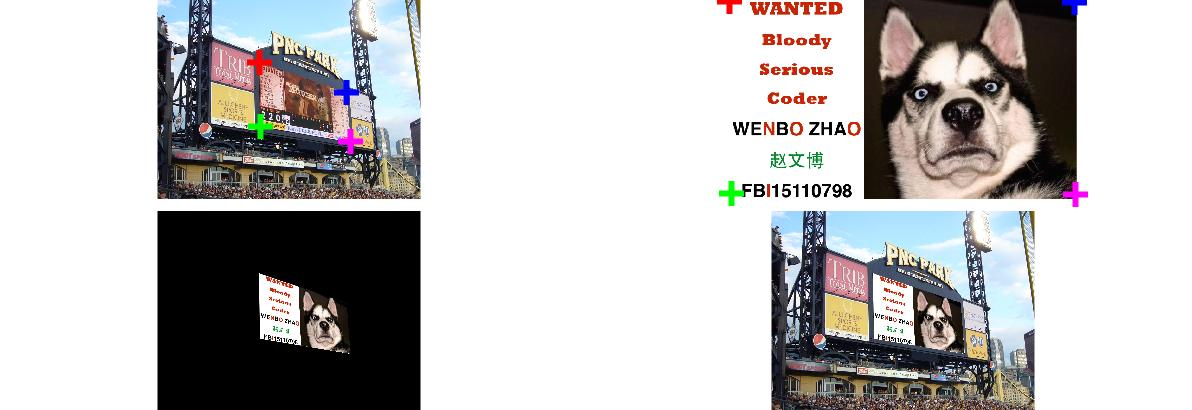
\includegraphics[width=0.9\linewidth]{q42checkerOutput.eps} %% edit here
\label{fig:q42checker}
\end{figure}

\end{enumerate}

\section{Panoramas (30pts)}

\subsection{(15pts)}

You're doing great! I think you've got this now.\\

\emph{RMSE = 1.2344.}\\

\begin{figure}[ht!]
\caption{q51checker output.}
\centering \includegraphics[width=0.9\linewidth]{q51_pano.eps} %% edit here
\label{fig:q42checker}
\end{figure}

\subsection{(15pts)}

You're doing great! I think you've got this now.\\

\begin{figure}[ht!]
\caption{q52checker output.}
\centering \includegraphics[width=0.9\linewidth]{q52_pano_extend.eps} %% edit here
\label{fig:q42checker}
\end{figure}
\end{document}
